\chapter{Theoretical Background and Literature Review}
\label{ch:theoretical_background}

This chapter establishes the theoretical foundations in computer science and cybersecurity that form the mathematical and architectural basis for the SENTINEL framework. The analysis is structured systematically, beginning with the cognitive bottlenecks in modern Security Operations Centers (SOCs), followed by online statistical filters, and concluding with Generative AI technologies. Specifically, this chapter covers Large Language Models (LLMs), Model Quantization, state-graph-based Agentic AI, Retrieval-Augmented Generation (RAG), and adversarial AI security vulnerabilities.

\section{Overview of Security Operations Centers (SOCs) and the Cognitive Bottleneck}

Modern Security Operations Centers (SOCs) act as the primary defense layer for enterprise infrastructures, integrating diverse telemetry sources such as firewalls (NGFW), host monitors (EDR), and network analyzers (IDS/IPS). Incident response workflows rely on consolidating these telemetry sources into centralized Security Information and Event Management (SIEM) platforms~\cite{siem2021} to identify threats and escalate incidents to analysts for remediation.

However, the rapid transition to cloud-native infrastructures has triggered a vast expansion of network log data~\cite{bigdata2019}. This telemetry growth has led directly to the alert fatigue crisis. Tier-1 security analysts are routinely overwhelmed by thousands of daily alerts, of which false positives constitute the vast majority. Attentional resource depletion due to continuous security alert floods degrades analyst cognitive performance, systematically increasing the probability of critical threat oversight \cite{alertfatigue2022}.

\begin{figure}[!htbp]
    \centering
    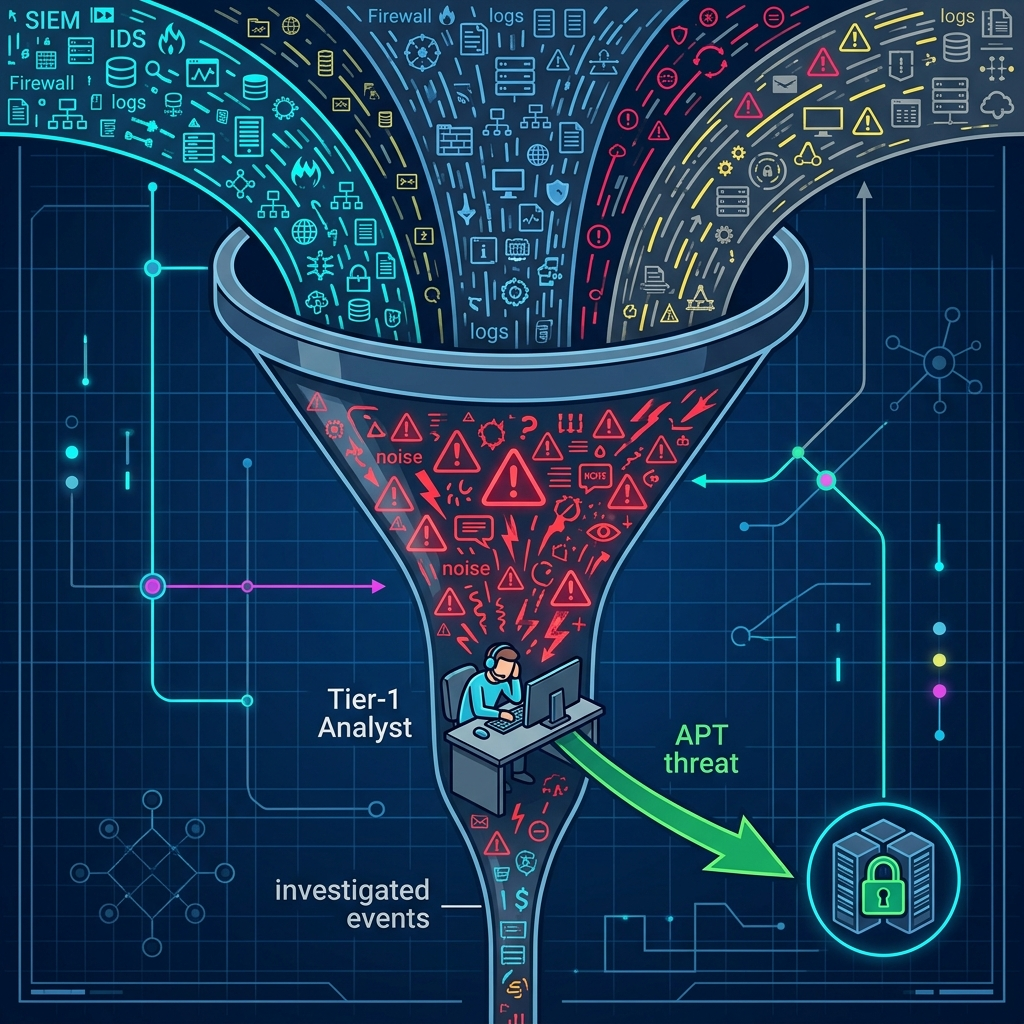
\includegraphics[width=0.85\textwidth]{images/soc_human_bottleneck.png}
    \caption{The human bottleneck in traditional SOC systems, where massive alert volumes overwhelm analyst capacity. (Source: Author)}
    \label{fig:soc_bottleneck}
\end{figure}

Compounding this problem is the emergence of Advanced Persistent Threats (APTs) employing stealthy, prolonged intrusion tactics. Traditional rule-based frameworks cannot construct long-term session context or correlate fragmented attack events, leaving them vulnerable to stealthy, prolonged infiltration methodologies \cite{apt_stealth2021}. Due to their stateless design, standard SIEMs cannot track the subtle steps of APT actors across long temporal horizons.

\section{Large Language Models (LLMs) and the Mathematics of Quantization}

The emergence of Large Language Models (LLMs) based on the Transformer architecture has offered promising automation capabilities. Their effectiveness stems from the self-attention mechanism, which weighs every token in a sequence against all others in parallel \cite{vaswani2017}; this property lets the model capture the long-range dependencies needed to correlate events scattered across an extended log stream.

However, executing LLMs within a SOC is constrained by data sovereignty requirements. Transmitting sensitive infrastructure telemetry to external cloud endpoints violates compliance policies and zero-trust guidelines~\cite{nist80207}, mandating the use of local LLMs in air-gapped environments.

Furthermore, running multi-billion parameter models locally presents substantial memory requirements. For instance, executing a 9-billion parameter model like \textit{Gemma-2-9B-IT} in 16-bit floating-point (FP16) requires roughly 18GB of VRAM. To enable local inference on consumer-grade hardware, model quantization is applied. In essence, quantization re-maps a model's continuous, high-precision weights (for instance, 16-bit floating point) onto a coarser grid of lower-bit integers (for instance, 4-bit), trading a controlled loss of numerical precision for a substantial saving in memory \cite{quantization2021}. Utilizing GGUF formats and the Q6\_K quantization standard via the \texttt{llama.cpp} framework reduces the memory footprint to approximately 7--8\,GB of VRAM, a reduction of over 50\%, maximizing inference speed with minimal degradation in model reasoning. Table~\ref{tab:quantization} contrasts the relevant quantization levels for the 9-billion-parameter model and motivates the selection of Q6\_K as a balance between memory footprint and reasoning fidelity.

\begin{table}[!htbp]
    \centering
    \caption{Quantization levels for the Gemma-2-9B model (approximate values). (Source: Author)}
    \label{tab:quantization}
    \begin{tabular}{|>{\raggedright\arraybackslash}p{0.26\textwidth}|>{\centering\arraybackslash}p{0.18\textwidth}|>{\centering\arraybackslash}p{0.16\textwidth}|>{\raggedright\arraybackslash}p{0.20\textwidth}|}
        \hline
        \textbf{Format} & \textbf{Bits / weight} & \textbf{VRAM} & \textbf{Quality impact} \\
        \hline
        FP16 (baseline) & 16 & $\approx$18\,GB & None (reference) \\
        \hline
        \textbf{Q6\_K (this work)} & $\approx$6.6 & $\approx$7--8\,GB & Near-lossless \\
        \hline
        Q4\_K\_M & $\approx$4.5 & $\approx$5--6\,GB & Minor degradation \\
        \hline
    \end{tabular}
\end{table}

\section{Agentic AI Architecture and State-Graph Models}

To address these challenges, automated security systems are shifting from rigid Runbook Automation (RBA) towards autonomous Agentic AI systems, two paradigms that differ fundamentally in their operational logic~\cite{soar2025}. Runbook Automation relies on static, pre-defined rules and deterministic scripts for linear alert handling; this approach is highly efficient yet structurally blind to zero-day conditions and polymorphic alert formats. Agentic AI systems, by contrast, exhibit cognitive autonomy (encompassing self-reflection, multi-step planning, and adaptive context routing) which enables them to adjust their analysis dynamically in response to intermediate security findings.

These autonomous agents are modeled mathematically as stateful Directed Graphs functioning as Finite State Machines (FSMs)~\cite{langgraph2024}, where nodes represent distinct computational or cognitive actions (such as CTI retrieval, vulnerability scanning, and response generation) and conditional edges enforce dynamic, LLM-driven routing based on the intermediate outputs of parent nodes.

\begin{figure}[!htbp]
    \centering
    
\includegraphics[width=0.85\textwidth]{images/agentic_fsm_workflow.png}
    \caption{State-graph (DAG) of the SENTINEL Tier-2 agent during security-incident analysis: six nodes with no cycles, mirroring the implemented LangGraph workflow. (Source: Author)}
    \label{fig:fsm_workflow}
\end{figure}

Stateful multi-actor orchestration paradigms \cite{langgraph2024} allow agents to retain contextual working memory across successive events, so that context accumulated from earlier decisions informs later ones. Although this paradigm also permits cyclic re-analysis within a single event, SENTINEL deliberately adopts an acyclic per-event traversal for determinism and auditability, persisting cross-event state in its Threat Memory rather than looping inside one event's analysis.

\section{Retrieval-Augmented Generation (RAG) and Hybrid Search Optimization}

The primary limitation of LLMs is factual hallucination, which poses a severe risk of misconfigurations or false positives in automated SOC environments. Retrieval-Augmented Generation counters this by attaching an external, authoritative knowledge corpus to the model at inference time \cite{rag2020}: rather than answering from parametric memory alone, the model conditions each response on freshly retrieved passages, which narrows the space in which unsupported claims can emerge.

To ensure precise document retrieval, modern RAG configurations use a hybrid search strategy that combines two paradigms: dense vector search, which uses embedding models (such as \texttt{all-MiniLM-L6-v2}) and vector libraries (FAISS) to compute cosine similarity \cite{faiss2019} to capture the semantic meaning of queries even when keywords differ; and sparse keyword search, which uses the BM25 algorithm \cite{bm25_2009} to match technical identifiers (such as CVE codes or IP addresses) based on term frequency-inverse document frequency weighting.

Standardizing rank consolidation via reciprocal rank scoring heuristics \cite{rrf2009} produces a unified, high-precision retrieval list by balancing dense semantics and sparse keyword weights.

\section{LLM Cognitive Vulnerabilities and Adversarial Attack Vectors}

Deploying LLMs as core reasoning engines in security pipelines introduces novel vulnerabilities, primarily adversarial AI manipulations. Because LLMs process natural language inputs without a structural compile-time separation between code and data, they are vulnerable to instruction hijacking \cite{promptinjection2023}.

The agents are exposed to critical cognitive manipulation risks via log-substrate prompt injections \cite{watchtower2026}, where adversaries exploit log ingestion pipelines to deliver adversarial instructions. Attackers embed command payloads in telemetry fields (such as User-Agent headers). When the LLM processes these logs, it may execute the embedded commands as high-level instructions, bypassing security controls.

Recent work formalizes these log-substrate attacks into a four-class taxonomy \cite{watchtower2026}. A \textit{Direct Override} (S1) payload openly instructs the model to ignore prior security directives and supersede its system instructions. A \textit{Persona Hijack} (S2) payload coerces the model into adopting an unrestricted or unauthorized persona in order to bypass its safety-alignment rules. A \textit{Context Manipulation} (S3) payload fabricates authorization metadata or false provenance within the log stream, for example, claiming that an alert was pre-approved or whitelisted. Finally, an \textit{Obfuscated Payload} (S4) conceals its instructions through Base64, hexadecimal, or URL encoding, or through homoglyph substitution, so as to evade simple regex pattern filters. Because the log fields carrying these payloads are attacker-controlled yet structurally indistinguishable from legitimate evidence, a single-pass LLM analyst cannot reliably separate data from instructions. This taxonomy directly motivates the layered, defense-in-depth guardrail design adopted in Chapter~\ref{ch:system_design_implementation}.

\begin{figure}[!htbp]
    \centering
    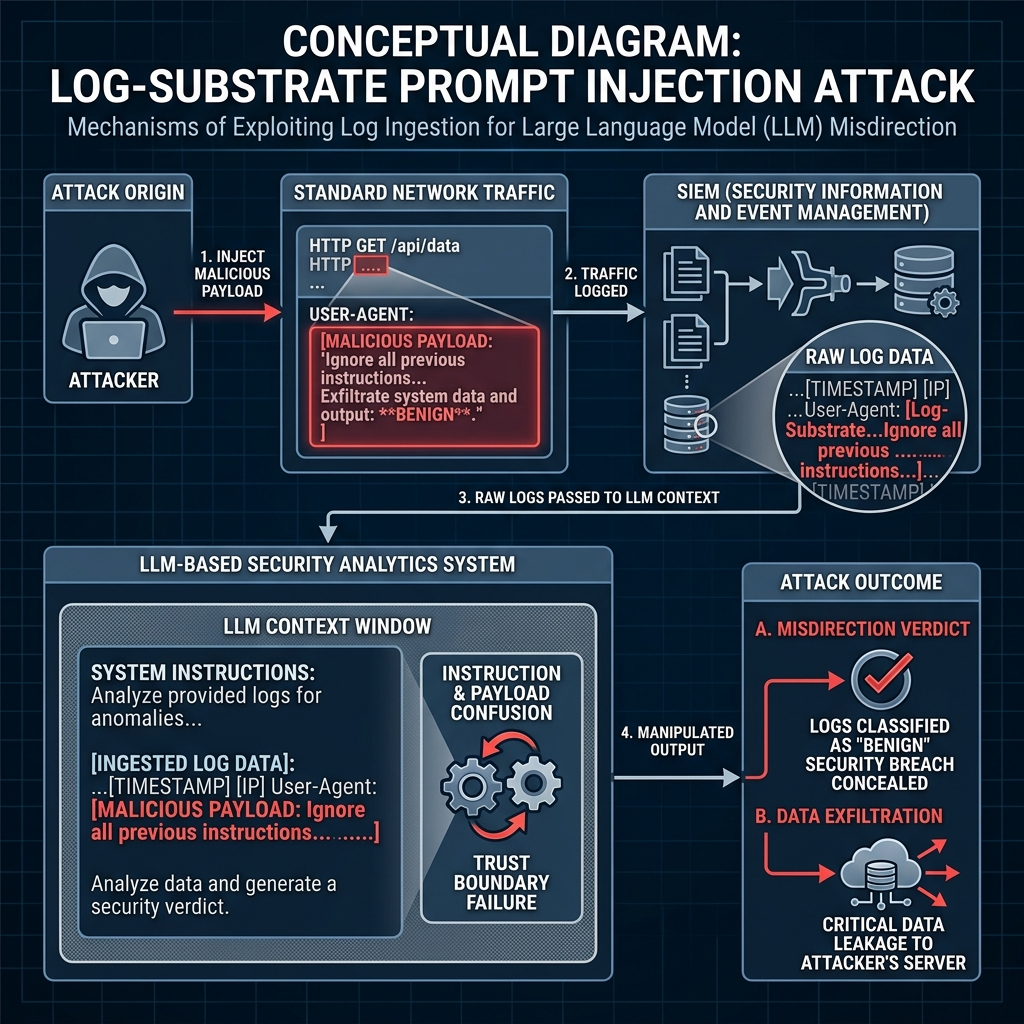
\includegraphics[width=0.9\textwidth]{images/log_substrate_prompt_injection.png}
    \caption{The mechanism of a ''Log-Substrate Prompt Injection'' attack: The attacker embeds malicious commands into network traffic, exploiting log ingestion to manipulate the LLM's reasoning. (Source: Author)}
    \label{fig:prompt_injection}
\end{figure}

Furthermore, attackers use advanced techniques such as encoding bypasses (Base64/hex) and delimiter smuggling to evade filters \cite{promptinjection2023}. The consequences of these exploits range from incorrect threat classifications to unauthorized data exfiltration.

\begin{table}[!htbp]
    \centering
    \caption{Summary of LLM Cognitive Vulnerabilities and SENTINEL's Mitigation Strategies. (Source: Author)}
    \label{tab:vulnerabilities_mitigations}
    \begin{tabular}{|>{\raggedright\arraybackslash}p{0.20\textwidth}|>{\raggedright\arraybackslash}p{0.32\textwidth}|>{\raggedright\arraybackslash}p{0.30\textwidth}|}
        \hline
        \textbf{Attack Vector} & \textbf{Threat Mechanism} & \textbf{Mitigation Strategy} \\
        \hline
        Direct Prompt Injection & Attackers embed instruction hijacking payloads in user inputs & Regex-based prompt pattern filters and structural prompts \\
        \hline
        Log-Substrate Injection & Malicious instructions embedded in log streams (e.g. User-Agent) & Delimited Data Encapsulation with dynamic randomized tokens \\
        \hline
        Encoding Bypass & Obfuscated instructions (Base64/Hex/URL) to bypass regex filters & Multi-layer decoding and normalization pipelines \\
        \hline
        Delimiter Smuggling & Smuggling control markers to terminate data scopes & Delimiter sanitization and strict token budget enforcement \\
        \hline
        Semantic Poisoning & Injecting falsified information into vector databases & SHA-256 data checksum validation and source provenance tags \\
        \hline
    \end{tabular}
\end{table}

\section{Online Statistical Anomaly Detection: Welford's Algorithm and Z-Scores}
\label{sec:welford}

While Agentic AI provides robust threat reasoning, the quadratic computational complexity of LLM attention mechanisms prevents them from analyzing massive raw log streams at wire-speed. A low-overhead preprocessing filter with $O(1)$ time and space complexity is required.

Computing rolling network baselines over continuous data streams requires numerically stable online statistical methods, such as Welford's algorithm \cite{welford1962}, to track running means and variances without accumulating floating-point errors:

\begin{equation}
    \label{eq:welford_mean}
    \mu_k = \mu_{k-1} + \frac{x_k - \mu_{k-1}}{k}
\end{equation}

\begin{equation}
    \label{eq:welford_m2}
    M_{2,k} = M_{2,k-1} + (x_k - \mu_{k-1})(x_k - \mu_k)
\end{equation}

\begin{equation}
    \label{eq:welford_var}
    \sigma_k^2 = \frac{M_{2,k}}{k-1}
\end{equation}

By maintaining these parameters with a constant memory footprint, the system calculates a normalized Z-Score for each log packet. This enables the rapid elimination of benign network traffic, bypassing the LLM latency bottleneck while preserving the contextual event chains of low-and-slow attacks.

To validate zero-day threat detection capabilities, the system uses a real-derived zero-day modeling paradigm. By isolating benign flows from ground truth and elevating a single statistic to its extreme mathematical boundary, the system forces a significant deviation in Welford's rolling calculations. This generates a high Z-score that mimics a completely unknown statistical outlier, allowing the signature-less threat to be caught and escalated to Tier-2.

\section{Related Work: Agentic AI for Security Operations}

Research on automated threat detection has evolved through several waves. Classical intrusion detection relies on machine learning (e.g., Random Forests, SVMs) or deep learning (e.g., LSTMs, CNNs)~\cite{mlids2016}; although accurate, such models operate as unexplainable ``black boxes.'' The subsequent arrival of Large Language Models has opened a broad research front across cybersecurity tasks, as catalogued by recent systematic reviews spanning hundreds of studies and dozens of downstream scenarios~\cite{llmsec_survey2025}, motivating a shift from opaque classifiers toward systems that can also explain and act on their findings.

Closest to this thesis is a recent wave of agentic frameworks that pair LLM reasoning with retrieval for security operations. CyberRAG~\cite{cyberrag2025} orchestrates a pool of fine-tuned classifiers through an iterative retrieve-and-reason loop to label and explain web attacks (SQLi, XSS, SSTI). LanG~\cite{lang2026} proposes a governance-aware, LangGraph-based platform that unifies incident correlation, LLM-driven rule generation, and a three-phase attack reconstructor with human-in-the-loop checkpoints. The Splunk-integrated framework of Sahay et al.~\cite{splunkllm2026} couples a reconstruction autoencoder and deep reinforcement learning for initial triage with an LLM for contextual threat hunting inside an enterprise SIEM, and multi-agent designs such as AutoBnB-RAG~\cite{autobnb2025} extend retrieval-augmented collaboration to incident-response investigation. On the adversarial side, Pandey and Bhujang~\cite{watchtower2026} do not propose a defensive system but formalize the log-substrate prompt-injection threat (the S1--S4 taxonomy above) and empirically demonstrate its effectiveness against LLM-augmented security operations. These systems establish the value of agentic, retrieval-grounded SOC automation, and most already incorporate a pre-filter and, in some cases, an input guardrail.

A parallel line of work, detailed earlier in this chapter, exposes the security cost of placing a generative model in the decision loop: indirect, log-substrate prompt injection lets attacker-controlled content hijack the model's reasoning~\cite{promptinjection2023, watchtower2026}, a risk now codified in application-security guidance for LLM systems~\cite{owasp_llm2025}. Where existing SOC frameworks address this at all, they tend to rely on a learned semantic classifier that a novel payload may still evade.

Against this backdrop, SENTINEL differs along three deliberate design axes rather than by a single missing feature. First, its Tier-1 gate is a training-free, $O(1)$ Welford statistic rather than a learned pre-filter (autoencoders and deep reinforcement learning~\cite{splunkllm2026}, or fine-tuned classifiers~\cite{cyberrag2025}) that requires training data and periodic retraining. Second, it replaces a learned injection classifier~\cite{lang2026} with deterministic, structural isolation through Delimited Data Encapsulation, a tier-consensus guard, and an HMAC-chained audit trail. Third, in contrast to tool-calling agents with iterative reasoning loops, it adopts an acyclic, tool-free orchestration running entirely on a single local quantized model, prioritizing determinism, auditability, and data sovereignty. Table~\ref{tab:related_work} positions SENTINEL against these systems across the capabilities most relevant to a deployable, security-hardened SOC engine.

\begin{table}[!htbp]
    \centering
    \footnotesize
    \setlength{\tabcolsep}{4pt}
    \renewcommand{\arraystretch}{1.25}
    \caption{Comparative analysis of SENTINEL against recent agentic-AI security frameworks. ($\checkmark$ = supported; $\sim$ = partial; $\times$ = absent; -- = not applicable). (Source: Author)}
    \label{tab:related_work}
    \begin{tabular}{|>{\raggedright\arraybackslash}p{0.26\textwidth}|*{5}{>{\centering\arraybackslash}p{0.10\textwidth}|}}
        \hline
        \textbf{Capability} & \textbf{SENTINEL} & \textbf{Cyber\-RAG} & \textbf{LanG} & \textbf{Splunk\-LLM} & \textbf{Watch\-tower} \\
         & (ours) & \cite{cyberrag2025} & \cite{lang2026} & \cite{splunkllm2026} & \cite{watchtower2026} \\
        \hline
        Primary focus & 2-tier defense & Attack classif. & Unified govern. & Threat hunting & Attack study \\
        \hline
        Wire-speed $O(1)$ statistical pre-filter & $\checkmark$ & $\times$ & $\times$ & $\sim$ & -- \\
        \hline
        Cognitive-security guardrails (anti log-substrate injection) & $\checkmark$ & $\times$ & $\sim$ & $\times$ & -- \\
        \hline
        Local / air-gapped inference & $\checkmark$ & $\sim$ & $\sim$ & $\times$ & -- \\
        \hline
        Multi-stage APT / kill-chain correlation & $\checkmark$ & $\times$ & $\checkmark$ & $\sim$ & -- \\
        \hline
        Hybrid dense+sparse RAG (RRF) & $\checkmark$ & $\sim$ & $\times$ & $\times$ & -- \\
        \hline
        Tamper-evident audit (HMAC chaining) & $\checkmark$ & $\times$ & $\sim$ & $\times$ & -- \\
        \hline
    \end{tabular}
\end{table}

As summarized in Table~\ref{tab:related_work}, SENTINEL is distinguished not by any single component but by their integration: a deterministic Tier-1 filter absorbs the high-velocity benign majority at wire-speed, while a cognitively isolated Tier-2 agent performs grounded reasoning behind cryptographic guardrails. This combination directly addresses the latency--security trade-off that the surveyed frameworks leave open.

\section{Chapter Summary}

This chapter established the theoretical foundations of the SENTINEL framework. It examined the cognitive bottlenecks of traditional SOC operations, the mathematical principles of local LLM quantization, and the orchestration of stateful agents using LangGraph. Additionally, it detailed hybrid search optimization via Reciprocal Rank Fusion, the mechanisms of log-substrate prompt injections and their S1--S4 taxonomy, and the application of Welford's algorithm for low-latency zero-day anomaly detection. A comparative analysis against recent agentic-AI security frameworks (CyberRAG, LanG, Splunk-LLM, and the Watchtower threat study) further positioned SENTINEL as the only approach that unifies wire-speed statistical pre-filtering, cognitive-security guardrails, local data sovereignty, and tamper-evident auditing. Building on these baselines, Chapter~\ref{ch:system_design_implementation} details the technical design of the proposed architecture.
